\chapter{视觉中的数学问题}

\section{最大似然估计}

\section{边缘化}	

\section{流形 — lie group}
\noindent\textbf{流形上的优化}:\\
\indent 位置、速度定义在欧式空间,可以直接进行优化处理。在欧式空间定义,特性是对加法操作封闭,比如$\textbf{t}_2=\textbf{t}_1+\bigtriangleup \textbf{t}$。但是姿态,只对乘法操作封闭$\textbf{R}_2=\bigtriangleup \textbf{R}*\textbf{R}_1$,需要在流形空间中进行优化。\\
简单说,流形是一个非线性空间,但是在局部空间内对其进行线性化,就可以用线性空间进行拟合。
\indent 对于一般的优化问题:
\begin{equation}
x=
\end{equation}


在流形上优化的好处:\\
1、有约束优化问题转化为无约束优化问题,如det(R)=1,有约束的优化问题会引入拉格朗日因子,优化变量维数会更高, 转换 李代数后,没有什么约束了,
\\
\\
\\
\\
\\
\\
\\

\subsection{李群对李代数的导数 }

对于$\xi\in SE(3)$定义\\
\begin{align}
	\xi^\wedge &=
	\left[ \begin{array}{c}   %该矩阵一共3列,每一列都居中放置
	\rho \\  %第一行元素
	\phi \\  %第二行元素
	\end{array}	\right] ^ \wedge = 
	\left[ \begin{array}{cc}
	   \phi^\wedge \quad  \rho \\
	    0^T        \quad  0
	\end{array} \right] \in R^{4x4},\rho,\phi\in R^3 \\	
	\xi^\curlywedge &=
	\left[ \begin{array}{c}   %该矩阵一共3列,每一列都居中放置
      	\rho \\  %第一行元素
    	\phi \\  %第二行元素
	\end{array}	\right] ^ \curlywedge = 
	\left[ \begin{array}{cc}
    	\phi^\wedge \quad  \rho^\wedge \\
    	0^T         \quad  \phi^\wedge
	\end{array} \right] \in R^{6x6},\rho,\phi\in R^3
\end{align}
其中$\rho$为平移分量,$\phi$为旋转分量。\\
\indent 假设某空间点p经过一次变换T(对应李代数$\xi$),得到Tp。现在,给T左乘一个扰动$ \bigtriangleup T = exp(\delta\xi ^ \wedge)$,假设扰动项的李代数为$\delta\xi=[\delta\rho,\delta\phi] ^ \wedge )$,那么:\\

\begin{equation}
\begin{aligned}
	\frac{\partial(Tp)}{\partial\delta\xi} &= \lim\limits_{\delta\xi\longrightarrow 0} \frac{exp(\delta\xi^\wedge)exp(\xi^\wedge)p - exp(\xi^\wedge)p}{\delta\xi} \\
	&\approx \lim\limits_{\delta\xi\longrightarrow 0} \frac{(I + \delta\xi^\wedge)exp(\xi^\wedge)p - exp(\xi^\wedge)p}{\delta\xi}\\
	&= \lim\limits_{\delta\xi\longrightarrow 0} \frac{\delta\xi^ \wedge exp(\xi^\wedge)p }{\delta\xi} \\
	&= \lim\limits_{\delta\xi\longrightarrow 0} \frac{
		\left[\begin{array}{cc}
	    	\delta\phi^\wedge \quad  \delta\rho \\
		    \textbf{0}^T      \quad  0
		\end{array}\right] 
		\left[\begin{array}{c}
	      \textbf{R}p+\textbf{t} \\
		  1
		\end{array}\right] }{\delta\xi} \\
	&= \lim\limits_{\delta\xi\longrightarrow 0} \frac{\left[\begin{array}{cc}
		\delta\phi^\wedge(\textbf{R}p+\textbf{t})+\delta\rho \\
		\textbf{0}^T    
		\end{array}\right] 
		}{\delta\xi} \\
	&= \lim\limits_{\delta\xi\longrightarrow 0} \frac{\left[\begin{array}{cc}
		-(\textbf{R}p+\textbf{t})^\wedge\delta\phi+\delta\rho \\
		\textbf{0}^T    
		\end{array}\right]
	}{\delta\xi} \\
    &= \left[\begin{array}{cc}
         \textbf{\textit{I}} \quad  -(\textbf{R}p+\textbf{t}) \\
         \textbf{0}^T        \quad  \textbf{0}^T 
       \end{array}\right] = (\textbf{T}p)^\odot
\end{aligned}
\end{equation}

\subsection{SE(3)的伴随矩阵}
李群伴随矩阵的作用,相当于实现李群乘法的交换律:
\begin{equation}
\textbf{T}exp(\xi^\wedge)=exp((Ad(\textbf{T})\xi)^\wedge)\textbf{T}
\end{equation}
稍加改变,用$\textbf{T}^{-1}$代替$T$得:(推导有待继续查,参考14讲11.1.2节)
\begin{equation}
exp(\xi^\wedge)\textbf{T} = \textbf{T}exp((Ad(\textbf{T}^{-1})\xi)^\wedge)
\end{equation}
伴随矩阵的解释,还可参照JingeTu的理解

\subsection{$\xi_{ij}$对 $\xi_i$、$\xi_j$的导数}
这部分的推到参考:\\
\indent 1)视觉slam14讲11.1.2节 Pose Graph的优化\\
\indent 2)JingeTu的博客https://www.cnblogs.com/JingeTU/p/9077372.html ,只是这里的推导方式不是很好,结合1)中的扰动法,推导过程如下。


\subsubsection{参考坐标系为全局坐标系时}
假设pose在世界坐标系w下定义,$\xi_i$、$\xi_j$即 $\xi_{wi}$、$\xi_{wj}$,则\\
\begin{align}
	\xi_{ij} = \xi^{-1}_{wi}\circ\xi_{wj}=In(exp((-\xi_{wi})^\wedge) exp( \xi_{wj}^\wedge))^\vee
\end{align}
对应的李群:\\
\begin{align}
\textbf{T}_{ij} = \textbf{T}_{wi}^{-1} \textbf{T}_{wj}= exp(\xi_{ij}^\wedge)
\end{align}
采用扰动法对$\xi_{wi}$、$\xi_{wj}$进行求导
\begin{equation}
\begin{aligned}
\xi_{ij}& = In(\textbf{T}_{wi}^{-1} * \textbf{T}_{wj})^\vee\\
        & =In((exp(\delta\xi_{wi}^\wedge)\textbf{T}_{wi})^{-1}  exp(\delta\xi_{wj}^\wedge)\textbf{T}_{wj})^\vee \\
        & =In(\textbf{T}_{wi}^{-1}exp((-\delta\xi_{wi})^\wedge)  exp(\delta\xi_{wj}^\wedge)\textbf{T}_{wj})^\vee \\
        & =In(\textbf{T}_{wi}^{-1}exp(-\delta\xi_{wi})  \textbf{T}_{wj}exp((Ad(\textbf{T}_{wj}^{-1})\delta\xi_{wj})^\wedge))^\vee \\
        & =In(\textbf{T}_{wi}^{-1} \textbf{T}_{wj} exp((-Ad(\textbf{T}_{wj}^{-1})\delta\xi_{wi})^\wedge)  exp((Ad(\textbf{T}_{wj}^{-1})\delta\xi_{wj})^\wedge))^\vee \\
        &\approx In(\textbf{T}_{wi}^{-1} \textbf{T}_{wj} [\textbf{I}-Ad(\textbf{T}_{wj}^{-1})\delta\xi_{wi} + Ad(\textbf{T}_{wj}^{-1})\delta\xi_{wj} ]) ^\vee\\
        &\approx In( exp(\xi_{ij}^\wedge) [\textbf{I}-Ad(\textbf{T}_{wj}^{-1})\delta\xi_{wi} + Ad(\textbf{T}_{wj}^{-1})\delta\xi_{wj} ]) ^\vee\\
        &\approx \xi_{ij}+\frac{\partial \xi_{ij}}{\partial \delta\xi_{wi}}\delta\xi_{wi}+\frac{\partial \xi_{ij}}{\partial \delta\xi_{wj}}\delta\xi_{wj}
\end{aligned}
\end{equation}
按照李代数上的求导法则,可求出$\xi_{ij}$对两个位姿 $\xi_i$、$\xi_j$的雅可比矩阵:
\begin{align}
\frac{\partial \xi_{ij}}{\partial \delta\xi_{wi}} &= -\mathcal{J}^{-1}(\xi_{ij})Ad(T_j^{-1})  \\
\frac{\partial \xi_{ij}}{\partial \delta\xi_{wj}} &= \mathcal{J}^{-1}(\xi_{ij})Ad(T_j^{-1})
\end{align}
由于se(3)上的左右雅可比$\mathcal{J}$形式过于复杂,通常取其近似。如果误差接近于零,就可以将它近似于$I$或者
\begin{align}
\mathcal{J}^{-1} \approx I+\frac{1}{2}\left[\begin{array}{cc}
\phi^\wedge \quad  \rho^\wedge \\
0      \quad  \phi^\wedge
\end{array}
\right]
\end{align}


\subsubsection{参考坐标系为局部坐标系时}
当参考坐标系选取为当前载体坐标系时,即$\xi_i$、$\xi_j$即 $\xi_{iw}$、$\xi_{jw}$,则\\
\begin{align}
\frac{\partial \xi_{ij}}{\partial \delta\xi_{iw}} &= \textbf{I}  \\
\frac{\partial \xi_{ij}}{\partial \delta\xi_{jw}} &= -Ad(\textbf{T}_{th})
\end{align}

%==========================================================
\section{矩阵正交化}
矩阵正交化本是矩阵问题,放在几何部分中,是因为想从几何的角度中来阐述。\\
本小节内容参见:https://blog.csdn.net/tengweitw/article/details/41174555、\\
https://blog.csdn.net/tengweitw/article/details/41775545\\

\subsection*{矩阵正交投影}

\begin{figure}[h]%%图
	\centering  %插入的图片居中表示
	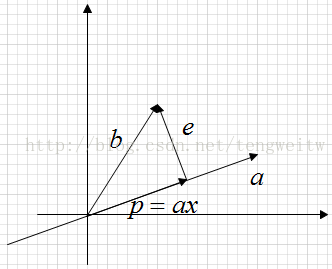
\includegraphics[width=0.7\linewidth]{math/img/1}  %插入的图,包括JPG,PNG,PDF,EPS等,放在源文件目录下
	\caption{向量b在向量a上的投影.}  %图片的名称
	\label{fig:mcmthesis-logo}   %标签,用作引用
\end{figure}
\noindent 图中,$\textit{\textbf{e}}=\textit{\textbf{b}}-\textit{\textbf{p}}=\textit{\textbf{b}}-x\textit{\textbf{a}}$,向量\textit{\textbf{e}}为投影残差\\
向量\textit{\textbf{a}}与向量\textit{\textbf{e}}垂直,\\ 
$\textit{\textbf{a}}^T\textit{\textbf{e}}=0 \longrightarrow \textit{\textbf{a}}^T(\textit{\textbf{b}}-x\textit{\textbf{a}})=0 \longrightarrow x\textit{\textbf{a}}^T\textit{\textbf{a}}=\textit{\textbf{a}}^T\textit{\textbf{b}} \longrightarrow x = \frac{\textbf{\textit{a}}^T\textbf{\textit{b}}}{\textbf{\textit{a}}^T\textbf{\textit{a}}}$\\
$x$是一个标量值,刻画了向量b投影到向量a上的长度。\\
\begin{center}
$\textbf{\textit{p}}=\textbf{\textit{a}}x = \textbf{\textit{a}}\frac{\textbf{\textit{a}}^T\textbf{\textit{b}}}{\textbf{\textit{a}}^T\textit{\textbf{a}}}$\\
\end{center}
\textbf{P}为投影矩阵,$\textbf{P}\textit{\textbf{b}}=\textit{\textbf{p}}$,则:
\begin{center}
$\textbf{P}=\frac{\textit{\textbf{a}}\textit{\textbf{a}}^T}{\textit{\textbf{a}}^T\textit{\textbf{a}}}$	
\end{center}


\subsection*{Gram-Schmidt正交化}
